
\chapter{Diskussion}

\begin{draft}

I detta kapitel diskuteras projektets metod, resultat,
vidareutvecklingsmöjligheter och etiska aspekter.

\end{draft}

\begin{binge}

De tre nedanstående ska vara nånstans i diskussion.

De domänspecifika språken modellerar områden snarare än att vara problemlösare.
\textit{Analys} exemplifierar detta väl. Det språket består av ett syntaxträd
över algebraiska uttryck samt operationer som derivering och integration. Med
hjälp av det kan man modellera uttryck och analytiska operationer på dem.
Däremot löser det inte problem åt en. Man kan med andra ord inte mata in en
differentialekvation och automatiskt få en lösning.

Hur bra våra moduler blev samt varför de inte är problemlösare utan modellerare
istället.

När områden kodades upp till domänspecifika språk var det långt ifrån alla gånger
det kunde göras på en meningsfullt sätt \todo{Expandera, Vad betyder
meningsfullt?}.

\section{Genomförandediskussion}

FÖRE DETTA TEORI- OCH METODVAL

Här ska vi vara kritiska till vårt teori- och metodval.

Sökande: När vi valde områden och gjorde läromaterial borde vi ha tydligt listat
de olika ''avsnitten'' i fysikkursen, och gjort ett DSL efter dom. Istället har
vi valt områden lite på måfå efter vad som verkat enklast att göra. Borde
planerat bättre för att anpassa de grundläggade DSLerna till vad som ingår i
fysikkursen. Så att mer relevant material och mer jämnt täckande av hela kursen.
Har lite att göra med avsnitt 1 i diskussion2.

Fast allt det ovanstående kanske är inaktuellt, för Åke sa ju att det säkert
hade räckt med ett par ordentliga områden, så att tankesättet förmedlas.

Skrivande: Pedagogsik aspekt i teori och metod bristande. Borde i teori gjort
mer allmän inläsning på pedagogik i allmänhet för vi kunde inte så mycket i
början. Sedan borde ha lagt större vikt på att pedagogiskt riktigt i metod när
vi skapade materialet. Svårt att veta om DSL+fysik pedagogiskt om materialet i
sig är dåligt pedagogiskt. DSL2016 skrev om interaktiv pedagogik. Hade vi kunnat
ha med eller liknande.

Utvärderingar: I samband med ovanstående, både om läromaterialet roligt/lärorikt
och om DSL+fysik pedagogiskt, borde haft större och längre utvärdering. I
allmänhet få möten och utvärderingar. Se vidareutveckling, om att kunde ha
större undersökningar...

--------

Detta ska anpassas in nånstans i det ovanstående

Fanns mycket i ARCS vi inte använder. Kanske därför inte kan förvänta oss att så
bra pedagogiskt.

Men projekets fokus var snarare av teknisk karaktär.

Egentligen har det väl varit skapandet som varit det lärorika och inte
användingen av det vi gjort? DSL2016 tyckte liknande här, så kan hänvisa till
dom.

Kan även hänvisa till dom att de la mycket tid på didaktik så mindre tid på
själva läromaterialet.

\section{Resultatdiskussion}

I detta kapitel diskuteras läromaterialet, kombinationen av domänspecifika språk
och fysik samt projektets relationen till liknande projekt.

\subsection{Läromaterialet}

En stor del av projektets mål var att skapa ett läromaterialet som både skulle
vara roligt och intressant att läsa. Vi skulle åstakomma detta genom att använda
oss av ARCS-metoden (?), användandet av lättsam text och roliga bilder för att
lätta upp materialet. 


----------

\subsection{Kombinationen av domänspecifika språk och fysik}

Ingress: En del av projketets mål var att diskutera kombinationen av
domänspecifika språk och fysik. I dessa tre avsnitt diskuterar vi därför
läromaterialets fokus på matematik och Haskell istället för fysik, vilka
fysikalsika områden som var lämpliga att göra domänspecifika språk till samt om
det finns en pedagogisk nytta i att kombinera de två. Diskussionen är till
största del baserad på våra erfarenheter efter att ha implementerat ett flertal
domänspecifika språk relaterade till fysik, men de är även baserade på
uppfattningar från testgruppen och Fäldt.


TODO: Allt detta ska kopplas mer till Åke-möten och testgrupp. Mycket är och ska
fortfarande vara våra egna erfarenheter, så inget fel på dem, men det andra ska
in också.

TODO: Ska också knyta an till VÅRT resultat om läromaterialet, när det gäller
vilka områden som var lämpliga.

Hur en kombination av domänspecifika språk och fysik ser ut är för oss inte
uppenbart. Går det att kombinera de två, och för vilka områden fungerar det bra
för? Är det lärorikt att presentera fysik ur ett
domänspecifikt-språk-perspektiv? Vi diskuterar här dessa frågor utifrån våra
egna erfarenheter från projektet och det vi lärde oss från utvärderingen med
testgruppen och mötena med Fäldt. 

\subsubsection{Om läromaterialets fokus på matematik och Haskell snarare än
fysik}
En stor del av läromaterialets fokus ligger på matematik och Haskell snarare än
fysik. Detta trots att läromaterialet är tänkt att handla om fysik. Varför är
det så?

En orsak till att ett stort fokus ligger på matematik är att fysik egentligen
bara är räkneexempel i matematik. Ta cirkulär centralrörelse som exempel. Att
beskriva en sådan rörelse hos en kropp görs med hjälp av vektorer och matematisk
analys. Fysik finns bara som en bakomliggande teori som dikterar vilka samband
som gäller. Själva räknandet görs sedan med matematik.

Detta är dock inte hela sanningen. Inom fysik ingår en stor del problemlösning,
till exempel att sätta upp och hitta krafter i mekanikproblem, utan att någon
matematik behöver blandas in. Denna typ av fysik är dock svår att göra
domänspecifika språk av, något som diskuteras djupare i
avsnitt~\ref{sec:lampligt}.

Läromaterialet innehåller även en hel del förklaringar av Haskell-teknisk
karaktär. Orsaken till detta är tvåfaldigt. För det första används avancerade
koncept inom Haskell som läsaren inte förväntas kunna sedan innan. Ett exempel
är typnivå-programmering. För att göra kopplingen mellan Haskell och fysik så
tydlig som möjlig behövdes fysikaliska dimensioner kunna likställas med, och
hanteras på samma sätt, som Haskell-typer.

För det andra är läromaterialets syfte inte enbart att lära ut fysik i sig, utan
även visa hur fysik kan modelleras i domänspecifika språk och dra paralleller
mellan fysik och domänspecifika språk. Av detta skäl blir det naturligt att det
''även'' ägnas en hel del förklaringar åt programkoden. Syftet är att väcka
intresse för fysik, inte att lära ut fysik. Ett sätt att göra det är att visa
dessa paralleller.

Är det rätt eller fel att ha en relativt liten tyngd på fysiken som projekets
läromaterial har? På den frågan har vi mer än ett svar. Man kan svara ja, med
hänvisning till de ovanstående skälen att det direkta syftet inte är att lära ut
fysik utan att väcka intresse. Man kan svara nej, och hävda att de
domänspecifika språken kan utformas på ett annat sätt som mer direkt knyter an
till fysikaliska koncept, till exempel ett syntaxträd för sammansättningen av
ett lutande plans komponenter. Vi tyckte dock det var svårt att göra på det
sättet, se avsnitt~\ref{sec:lampligt}. Detta är dock en
vidareutvecklingspotential, att undersöka huruvida det går att göra det på ett
bra sätt.

Man kan också svara nej på frågan av ett annat skäl, nämligen att fysiken i sig
bör vara det främsta fokuset. Detta skulle dock innebära en helt annan form på
läromaterialet. Vi menar att det skulle vara svårt att väva in domänspecifika
språk på ett meningsfullt sätt om de samtidigt skulle vara i skymundan. Ett
läromaterial med större fokus på fysik bör i så fall enbart handla om fysik. En
utförligare diskussion om detta finns i avsnitt~\ref{sec:bara_fysik}.

\textbf{------------------------------}

Målet med läromaterialet var att lära ut fysik på ett roligt och lättförståeligt
sätt. Dock syns det vid läsning av materialet att det stora fokuset lagts på att
förklara och lära ut matematik och Haskell. Varför blev det så? Vi menar att det
finns många anledningar till detta. 

\begin{figure}[tph]
  \centering
  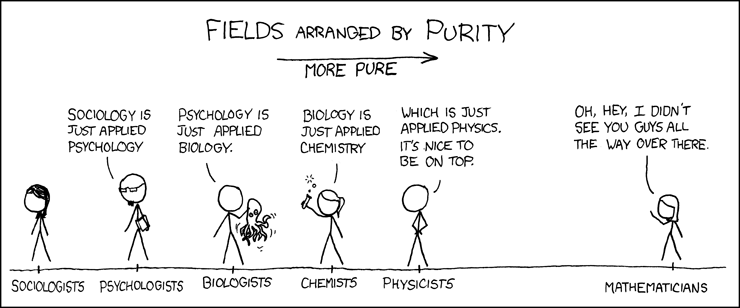
\includegraphics[width=0.75\textwidth]{figure/purity.png}
  \caption{XKCD:s beskrivning av samma problem.}
\end{figure}

Problemet med att prata om en egen implementation av fysik är att fysik inte är
ett helt eget område. Det är snarare så att fysik kan ses som applicerad
matematik, att fysik använder matematiken för att beskriva det fysikaliska
universum vi lever i. Det blir därför naturligt att när den faktiska
implementationen av dessa beskrivningar och lagar sker, så sker de med hjälp av
matematiken. Att ett stort fokus läggs på matematiken är alltså bara en
konsekvens av fysiken i sig själv.

Såklart ingår det ochså en hel del problemlösning inom fysik, den faktiska
applikationen av de beskrivningar och lagar som matematiken ger oss. Men
problemlösning är något som vi tycker är svårt och problematiskt att modellera
som ett domänspecifikt språk, något som diskuteras djupare i
avsnitt~\ref{sec:lampligt}.

Anledningen till att ett stort fokus läggs på Haskell är att eftersom
implementationen av fysik ibland använder sig av koncept som inte alltid är
kända för en läsare med endast en grundläggande förståelse för Haskell måste
dessa koncept förklaras grundligt så att ingen förståelse går förlorad. Och
eftersom ett syfte med läromaterialet var väcka intresse hos läsaren med
bakgrund inom Haskell så ville vi lägga fokus på att tydligt visa på
parallellerna mellan funktionell programmering, matematik och implementationen
av fysik. 

Vi hävdar alltså att fokuset inte enbart lagts på fysik pågrund av att det inte
är så fysik fungerar och att det är lika viktigt att förklara Haskell. Men måste
det vara så? Det kan mycket väl vara så att detta fokusskifte har skett pågrund
av hur vi valde att genomföra projektet. I ett tidigt skede valde vi söka efter
områden som vi ansåg vara fristående och väl avgränsade~\ref{sec:konstruktion},
och implementera dessa var för sig. Utan tvekan har detta sätt att påbörja
projektet påverkat allting som kom därefter, om vi istället hade utvecklat
läromaterialet som en kombination av olika områden från början hade det kanske
inte varit lika främmande att även baka in problemlösning i detta och på så sätt
fått in ett ordentligt fysikperspektiv. 

Även tidigare än så går det att vara kritisk till projektets utformning. Varför
valdes Haskell som implementationsspråk? Vi hävdar i teorin~\ref{sec:syntax} att
Haskells typer och fokus på mönstermatchning gör det idealt för implementering
av domänspecifika språk.  Men betyder det att det är idealt för implementering
av fysik? Kanske ett objektorienterat språk som Java hade passat bättre. Att
använda ett språk som inte har en lika stark koppling till ren matematik som
Haskell har hade kanske lett till att det stora fokuset inte låg på matematiken
bakom fysiken, utan istället på fysiken framför matematiken.

\subsubsection{Vad för slags områden är DSLs lämpligt att göra för?}
\label{sec:lampligt}

TODO: Hänvisa mer till resultat. Att av dessa skäl är inga DSLs för fysik.

TODO: Se AIFTTM i bedömningskriterier. Här kan vi knyta an till metod genom: den
klassificiering som gjordes (grund/komposit)- att den ledde till denna tudelning
om inte så fysikaliska DSLs, 

Under projektets gång gjordes flera experiment för att se hur man kunde göra ett
domänspecifikt språk för ett område. Det visade sig att visa områden var
lämpligare än andra. Till exempel var analys och vektorer områden som vi ansåg
väl lämpade, medan andra som till exempel lutande plan och termodynamik var
mindre lämpade.

Vad har de lämpliga områdena gemensamt? De gemensamma dragen är att de är
matematiska, har en fix struktur och består av ``data och operationer''.
Tabell~\ref{tab:data_och_ops} visar några exempel på områden med sina data och
operationer.

\begin{table}[tph]
\centering
\caption{Exempel på data och operationer i några domänspecifika språk.}
\label{tab:data_och_ops}
\begin{tabular}{@{}l|l@{}}
\toprule
DSL / data & Exempel på operationer \\ \midrule
Dimensioner & Multiplikation, division \\
Vektorer & Addition, skalärprodukt \\
Analys, funktioner & Derivera, multiplicera \\ \bottomrule
\end{tabular}
\end{table}

Varför gör dessa drag att de är lämpliga att göra domänspecifika språk för?
TODO: Matematiska: man modellerar syntaxen

Den fixa strukturen kombinerat med data och operationer gör det enkelt att
modellera dessa områden med datatyper i Haskell. Datatyper har nämligen också en
fix form. Dessutom blir relationen mellan data och operationer i Fysik och
datatyper och funktioner i Haskell väldigt tydlig. En operation/funktion
resulterar sedan i data av samma slag som innan \todo{Som innan?}.

Denna strukturella likhet gör modellerandet och manipulerandet av data enkel att
genomföra rent tekniskt. Men den innebär också en pedagogisk vinst. Genom att ha
strukturerat upp fysik tydligt i Haskell blir det förhoppningsvis enklare för
läsaren att förstå hur datan hänger ihop rent fysikaliskt. Och även hur
relationerna mellan olika datatyper och funktionerna som dyker upp i
läromaterialet direkt kan översättas till relationer inom fysik.

I kontrast till dessa lämpliga områden står mindre lämpliga områden (eller
åtminstone områden som vi inte lyckades göra något bra av). Som nämndes tidigare
är termodynamik och lutande plan exempel på mindre lämpliga områden. Vad har
dessa områden för gemensamma drag?

Ett gemensamt drag som gör dem svåra att göra domänspecifika språk av är att de
består av en samling teoretiska samband. För det lutande planet är det till
exempel $a = g \cdot \sin(v)$, som illusteras i figur~\ref{fig:lutande_plan}.

\begin{figure}[tph]
  \frame{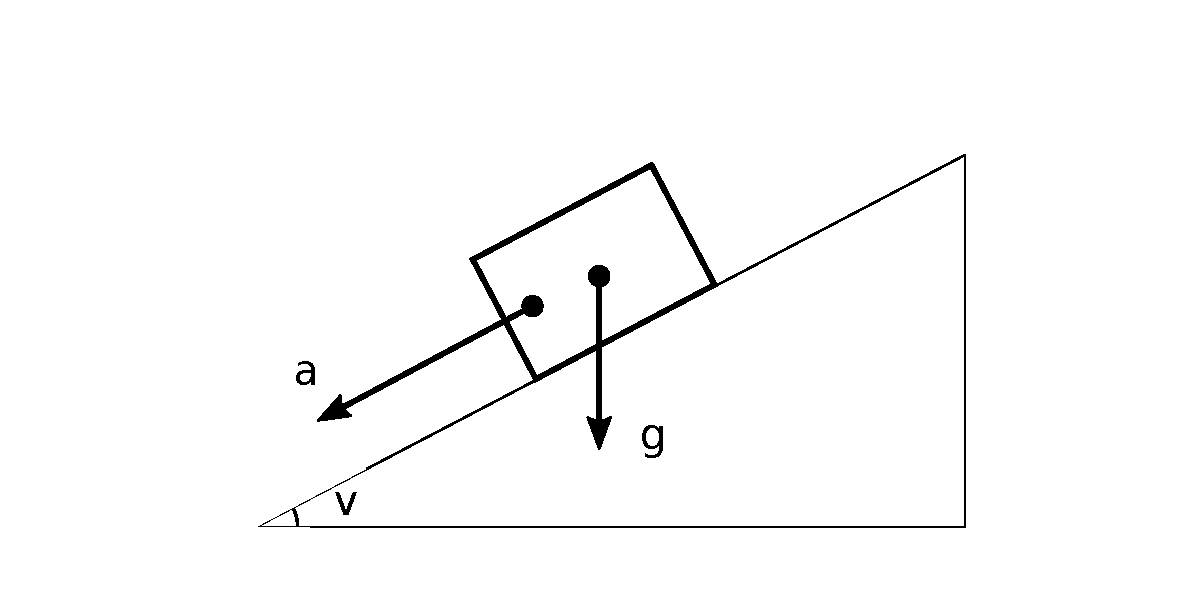
\includegraphics[width=\linewidth]{figure/Lutande_plan.pdf}}
  \caption{Den variant av lutande plan som referas till i exemplet i texten. $a$
  är en lådas acceleration längs med planet, $g$ är tyngdacceleration och $v$ är
  vinkeln. Friktionen antas vara försumbar.}~\label{fig:lutande_plan}
\end{figure}

Teoretiska samband av det slaget relaterar olika egenskaper i systemet.
Visserligen kan man modellera samband och ekvationer som ett domänspecifikt
språk, men vi menar att nyttan inte blir stor med det. Det man kan göra är att
programmera en ekvationslösare. Men den hade behövt vara både mekanisk och
komplex. Den skulle alltså skilja sig drastiskt från hur man löser problem för
hand och skulle vara svår att förstå. Alldeles för mycket fokus skulle hamna på
algoritmer istället för fysik.

När det kommer till lutande plan och liknande områden är nyckeln att visserligen
känna till vilka samband som gäller, men det framförallt att veta när man ska
använda dem och hur man tillämpar dem på olika typer av uppgifter. Vi behandlar
därför områden som lutande plan genom att lösa exempeluppgifter modellerade i de
tidigare domänspecika språk. De tidigare språken tillhandahåller de matematiska
verktyg som behövs för att koda upp lösningar av problem.


TODO: Kanske avsluta med att poängtera skillnaderna mellan lämpliga och mindre
lämpliga.

Och vad är skillnaden mellan dessa två kategorier av områden?

Den viktiga skillnaden är att t.ex. analys har tydlig data och operationer 
medan problemlösning som lutande plan består av ett antal samband som används
beroende på behov. Dessa samband består då av koncept som redan är modellerade i
andra avsnitt och själva skrivandet av den koden bidrar inte med någon ny
kunskap som inte redan täcks av vanlig kurslitteratur inom fysik.

\subsubsection{Gör DSLs så att fysik blir mer lättförståeligt eller
intressant?}~\label{sec:bara_fysik}

TODO: Se AIFTTM i bedömningskriterier. Här kan knyta an till metod genom att
påpeka att inte så ordentlig undersökning med testgrupper med och utan att ha
läst detta. Inga intervjuer med folk om de tyckte läromaterialet var intressant
och om de tyckte det gjorde fysik intressantare.

En del av detta blir överlapp med "Metod och teorival" i disk1. Det mesta kanske
ska stå där, och här hänvisas till dit?

TODO: Åke-möte2 gav viktiga insikter här som vi kan hänvisa till, utan att
samtidigt få det att verka som Åke otvetydigt sagt att detta är bra utan att han
verkar tycka att det kan vara något, efter en kort titt på det. För att "låta
hans rygg vara fri".

TODO: Att vissa var olämpliga kan ses som ett oväntat resultat.

TODO: Relation till annat liknande är bl.a. DSL2016 och DSLsofMath. Bra att få
med.

Är det pedagogiskt att lära ut fysik genom att presentera den med hjälp av
domänspecifika språk? Väcker det intresse för fysik? Tillförde de domänspecifika
språken något i detta läromaterial eller hade det varit bättre att enbart hålla
sig till fysik? Dessa tre frågor diskuteras nedan.

Domänspecifika språk kan betraktas som ``tools for thinking'' (gör detta till
ett citat av Patrik). Med det menas att domänspecifika språk kan användas till
att struktutera ett område så att det blir enklare att få en överblick och
förstå det. Dimensioner i läromaterialet är ett exempel på detta, se även
avsnitt \ref{sec:grund_impl}. Där konstateras att en godtycklig dimesion kan
skrivas som de sju grunddimensionerna med tillhörande exponenter. Eftersom
dimensionerna måste defineras så tydligt att det går att göra ett program av det
tvingas man att ge struktur till dem. Det ger ett nytt, välstrukturerat och
förhoppningsvi enklare sätt att se på dem, vilket vi själva tycker är
meningsfullt.

År 2016 genomfördes ett kandidarbete på Chalmers liknande detta. \cite{DSL2016}
Det kandidatarbetet resulterade också i ett läromaterial. Skillnaden är att det
handlade om signallära medan detta handlar om fysik. Grundidėn är dock densamma:
att använda domänspecifika språk för att ge struktur till ett annat område.

En annan aspekt är att när de domänspecifka språken används till fysikalisk
problemlösning måste det ske enligt de regler som ställdes upp när det
domänspecifika språken definerades. Det går med andra ord inte att fuska och ta
genvägar i problemlösningen. Detta tankesätt tycker Fäldt, se avsnitt
\ref{sec:res_ake}, är en bra grej som förmedlas med att presentera fysik på
detta sätt. Studenten skolas in i att tänka i rigorösa och kompletta banor.

% Viktigt att något kritiskt, som det nedanstående, är med
Det som talar emot domänspecifka språk när det kommer till fysik är den stora
del av problemlösning som ingår i fysik. Det har att göra med deras olika natur.
Domänspecifka språk har en entydig och fyrkantig struktur medan problemlösning
handlar om kreativitet och nytänkande. Eftersom en stor del i fysik är just
problemlösning kan denna del inte fångas upp med domänspecifika språk. Det
skulle till och med kunna vara en nackdel att kombinera domänspecifka språk och
fysik om det leder till att man tänker alltför fyrkantigt kring fysik. Vi anser
dock att domänspecifika språk har ett värde ihop med fysik just för dessa
strukturgivande möjligheter, även om inte alla aspekter av fysik kan täckas.
Dessutom kan man tänka sig att det finns ett värde i ett fånga upp den kreativa
problemlösningen med ett fyrkantigt system och på så sätt stoppa problemlösaren
från att göra misstag, på ett förenklat sätt kan man säga att så länge
typsystemet inte klagar så löser man problemet på ett korrekt sätt.

--------

Från ett annat perspektiv kan man betrakta domänspecifika språk som ett sätt att
\textit{väcka intresse} för fysik. Tycker man att domänspecifika språk är roligt
men inte fysik skulle en överbryggning av dem kunna göra att man tycker fysik
blir roligare. Detta kan göras genom att man ser parallellerna mellan
domänspecika språk och fysik. Ett exempel är typsystemet i Haskell och
dimensioner i fysik. I bägge världarna får inte olika typer respektive
dimensioner adderas, och vid operationer behandlas de på liknande sätt. Denna
likhet påvisades i läromaterialet genom att implementera fysikaliska dimensioner
i Haskells typsystem, se avsnitt \ref{sec:res_laromaterial}. Denna tanke stöds
av att även testgruppen tyckte läromaterialet var ett intresant sätt att
presentera fysik på, se avsnitt \ref{sec:res_test}. Nyttan med ett större
intresse för fysik är att man då förhoppningsvis är mer motiverad att lära sig
fysik för att klara fysikkurser i skolan. 



Hittills har domänspecifika språk framförts som ett sätt att strukutera fysik
och göra den intressantare. Projkets läromaterial är ett exempel på ett sådant
försök. Men läromaterialet har även haft två andra drag, förutom domänspecifika
språk, som skiljer sig från traditionell fysikundervisning, nämligen ett
lättillgängligt språk och en nogrann genomgång av koncepten. Hade inte detta
räckt? Hade fysiken i sig inte kunnat förklarats bättre om den haft allt fokus?

Vi tror att svaret på båda dessa frågor är ja, med vissa reservationer. Ett
läromaterial om renodlad fysik med ett lättsamt språk och nogrann förklaring av
koncepten hade säkert varit uppskattat. Khan Academy är ett sådant
exempel.\cite{khan}. En annan fördel hade varit att en större målgrupp kan nås.
Dock känner vi att om man väl är intresserad av domänspecifka språk hade det
varit både tydligare och intressantare att kombindera dem med fysik, än att bara
presentera fysik. Dessutom kan ju själva kombinationen i sig vara intressant,
och inte bara fysiken.

TODO: Vad testgruppen tyckte bör stå nånstans. Men var?

Halvvägs genom projektets gång hade vi ett möte med en annan grupp som också
utvecklade ett läromaterial. Under mötet hade vi ett utbyte av idéer och tankar
och tog även tillfället i akt att läsa och testa varandras material. Den
generella feedbacken vi fick var vi absolut var inne på rätt spår och att
läromaterialet till största del uppfyllde vårt mål med att göra läromaterialet
både intressant och lättillgängligt. Och även om de inte hade någon tidigare
erfarenhet av DSLer så tyckte de inte att det var något problem att ta till sig
koncepten som vi beskrev. Även om detta inte kan ses som något officielt test av
vårt läromaterialet eftersom testgruppen var så liten kanske det kan ses som en
fingervisning att vi är på rätt spår.

Testgruppen tyckte det var ett intressant sätt.

TODO: På ett smidigt sätt väver vi in DSL2016 och DSLsofMath.

TODO: Även LYAH liknande

Det finns flera andra projekt som resuterat i liknande 

\section{Vidareutvecklingsmöjligheter}

Läromaterialet innehåller domänspecifika språk för de \textit{matematiska}
områdena analys och vektorer. Dessa områden används sedan för att koda upp och
lösa uppgifter av mer \textit{fysikaliska} slag, till exempel lutande plan. Med
andra ord görs inga domänspecifika språk för fysik i sig. En vidareutveckling
hade därmed varit att göra precis det, att inte bara tillämpa matematiska
domänspecifika språk utan göra fysikalsika domänspecifika språk. Det kan vara
saker som ett syntaxträd för ett lutande plans komponenter. Det kan vara ett
syntaxträd för vilka krafter som verkar på fysikalsika kroppar i mekanikproblem.
Det kan till och med vara ett domänspecifikt språk för något så abstrakt som
fysikalisk problemlösning i allmänhet. Vi har dessvärre ingen aning hur det
skulle kunna se ut. Men av just detta skäl tror vi det hade varit väldigt
intressant att se hur ett mer fysik-orienterat domänspecifikt språk kan se ut.

En annan möjlig vidareutveckling är att göra en rigorös studie kring de
pedagogiska aspekterna kring kombinationen av fysik och domänspecifika språk.
Detta projekt innehöll enbart en mindre sådan studie. Det som kan vara
intressant att undersöka är om studenter tycker att fysik blir intressantare
genom en kombination av detta slag och kanske därför studerar mer i fysikkursen.
Eller kanske om de rent av blir bättre på fysik i sig genom att fysik
presenterats på detta sätt, det vill säga att ett läromaterial av detta slag
skulle kunna fungera istället för traditionell undervisning inom fysik. Givetvis
skulle kompletering av läromaterialet behöva göras så att det är heltäckande.

Slutligen kan det befintliga läromaterialet byggas vidare på. I sin nuvarande
form behandlas varken termodynamik eller vågrörelselära något alls. Dessutom lär
det finnas aspekter inom den klassiska mekaniken som fattas.

TODO: Kanske kan vara intressanta att ha ett projeket som använder DSL till
fysik för att visa korrekthet, på det sätt Jeff var inne på. Alltså att man kan
göra annat än bara läromaterial som de två senaste kandidatarbetena varit.

\section{Etiska aspekter}

En bakomliggande tanke vi haft genom hela projektet är att läromaterialet ska
vara tillgängligt för alla. Därav har vi valt att publicera det på en hemsida.
Denna hemsida använder grundläggande HTML och CSS samt javascript. Javasript är
dock inget krav för funktionalitet. Eftersom hemsidan är lättviktig bör den
fungera väl även på gamla datorer och telefoner, till skillnad från tunga
PDF-filer och många moderna hemsidor.

Tanken om tillgänglighet ligger även bakom valet att låta källkoden var fritt
tillgänglig. Visserligen \textit{är} läromaterialet i princip hela källkoden, så
har man läromaterialet har man källkoden. Att ha källkoden dirket har dock
fördelar som att man kan följa med i versionshistoriken, man kan se kommentarer
och alternativa implementationer som inte syns i den slutgiltiga produkten samt
att det blir enklare att modifera källkoden och man inte behöver
reverse-enginnera hemsidan. Det handlar om att visa att man är positiv till att
andra tittar hur man gjort och låta andra bygga vidare på ens skapelser. Genom
att sluta oss till skaran som tillämpar öppen källkod hoppas vi att fler inom
samhället i stort ska gå över till denna modell.

Valet att skriva på engelska har också att göra med tillgängligheten. Fler kan
engelska än svenska. Så på detta sätt kan läromaterialet komma fler till gagn.

Roligt <-- vet ej hur ska få in bra.

Om Hemsidan:
  Det är lite intressant ur pedagogik-aspekten. Kan det
  kanske vara lättare/roligare att lära sig om sidan är fin och
  lättläst? Att javascript inte krävs gör att sidan kan visas ordentligt
  även om man sitter i U-land med dålig/gammal/billig telefon.

\end{binge}
